\documentclass[12pt, twoside]{article}
\usepackage[letterpaper, margin=1in, headsep=0.5in]{geometry}
\usepackage[english]{babel}
\usepackage[utf8]{inputenc}
\usepackage{amsmath}
\usepackage{amsfonts}
\usepackage{amssymb}
\usepackage{tikz}
\usetikzlibrary{quotes, angles}
\usepackage{graphicx}
%\usepackage{pgfplots}
%\pgfplotsset{width=10cm,compat=1.9}
%\usepgfplotslibrary{statistics}
%\usepackage{pgfplotstable}
%\usepackage{tkz-fct}
%\usepackage{venndiagram}

\usepackage{fancyhdr}
\pagestyle{fancy}
\fancyhf{}
\renewcommand{\headrulewidth}{0pt} % disable the underline of the header

\fancyhead[RE]{\thepage}
\fancyhead[RO]{\thepage \\ Name: \hspace{3cm}}
\fancyhead[L]{BECA / Dr. Huson / Geometry 10th Grade\\* Unit 2: Midpoints and distance \\ 
19 September 2019}

\begin{document}
  \subsubsection*{2.4 Homework: Solving for lengths}
  \begin{enumerate}


\item Find the area of $\triangle ABC$. The altitude $h$ of the triangle is $7 \frac{1}{4}$ centimeters and the base $AB=12 \frac{1}{2}$ cm.\\[0.5cm]
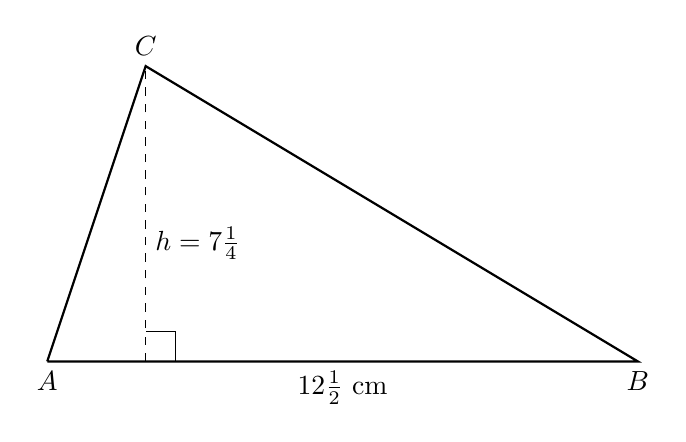
\begin{tikzpicture}[scale=1.25]
  \draw [thick]
    (2,0)node[below]{$A$}--
    (8,0)node[below]{$B$}--
    (3,3)node[above]{$C$} --(2,0);
 \draw [dashed] (3,0)--(3,3);
 \draw (3,0)++(0.3,0)--++(0,0.3)--+(-0.3,0);
 \node at (3,1.2)[right]{$h=7 \frac{1}{4}$};
 \node at (5,0)[below]{$12 \frac{1}{2}$ cm};
\end{tikzpicture} \vspace{1.0cm}

\item Given the rectangle $ABCD$ shown below, with $AB=17$. If the area of the rectangle is 102, find $BC$.
\begin{flushleft}
\begin{tikzpicture}[scale=0.8]
  \draw [-, thick] (0,0)--(8,0)--(8,3)--(0,3)--cycle;
  \draw [fill] (0,0) circle [radius=0.05] node[left]{$A$};
  \draw [fill] (8,0) circle [radius=0.05] node[right]{$B$};
  \draw [fill] (8,3) circle [radius=0.05] node[right]{$C$};
  \draw [fill] (0,3) circle [radius=0.05] node[left]{$D$};
  \node at (8.5, 1.5){?};
  \node at (4, -0.5){17};
\end{tikzpicture}
\end{flushleft}
\vspace{1.5cm}

\item Given that the area of $\triangle KLM$ is 24 and the base $KL=12$. Find the altitude $h$ of the triangle.\\[0.5cm]
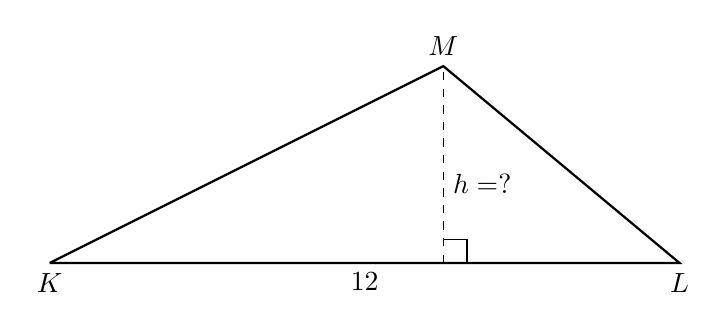
\begin{tikzpicture}[scale=1]
  \draw [thick]
    (-5,0)node[below]{$K$}--
    (3,0)node[below]{$L$}--
    (0,2.5)node[above]{$M$} --(-5,0);
 \draw [dashed] (0,0)--(0,2.5);
 \draw (0,0)++(0.3,0)--++(0,0.3)--+(-0.3,0);
 \node at (0,1)[right]{$h=?$};
 \node at (-1,0)[below]{$12$};
\end{tikzpicture} \vspace{1.0cm}

\newpage
\item Given $\overleftrightarrow{WZ}$ as shown on the number line. \\[20pt] % Midpoint
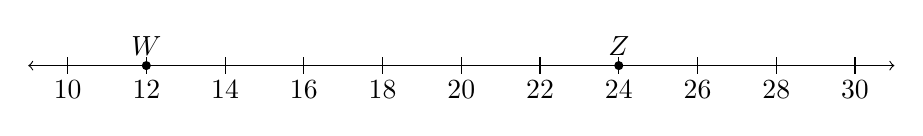
\begin{tikzpicture}[scale=0.5]
  \draw [<->] (9,0)--(31,0);
  \foreach \x in {10, 12,...,30} %2 leading for diff!=1
    \draw[shift={(\x,0)},color=black] (0pt,-6pt) -- (0pt,6pt) node[below=5pt]  {$\x$};
    \draw [fill] (12,0) circle [radius=0.1] node[above] {$W$};
    \draw [fill] (24,0) circle [radius=0.1] node[above] {$Z$};
\end{tikzpicture} \\ \vspace{1cm}
Mark and label two points $X$ and $Y$ that trisect $\overline{WZ}$. \vspace{1cm}

\item Given $\overline{PQR}$, with $PQ=4x-4$, $QR=2x+3$, and $PR=5x+9$. Find ${PR}$.\\
Complete all the steps for full credit. \smallskip
\vspace{9cm}

\item Given $\overline{DEFG}$, $DE=3 \frac{1}{3}$, $EF=4 \frac{2}{9}$, and $FG= 2 \frac{4}{9}$. (diagram not to scale)\\ [0.25cm]
  Find ${DG}$.\\[.5in]
      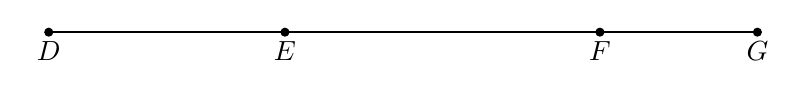
\begin{tikzpicture}
        \draw [-, thick] (0,0)--(9,0);
        \draw [fill] (0,0) circle [radius=0.05] node[below]{$D$};
        \draw [fill] (3,0) circle [radius=0.05] node[below]{$E$};
        \draw [fill] (7,0) circle [radius=0.05] node[below]{$F$};
        \draw [fill] (9,0) circle [radius=0.05] node[below]{$G$};
      \end{tikzpicture}
      \vspace{4cm}

\end{enumerate}
\end{document}
